\chapter{Waves}

%
%  SECTION 5.1 - Gravity and Capillary Waves
%

\section{Gravity and Capillary Waves}


% 5.1.1 - Surface Waves (examples of waves, generation of surface waves, gravity and capillary waves and both combined, drawing of a wave and definitions)

\subsection{Surface Waves}

We turn our attention now to the \emph{interface} between two fluids -- in our discussion here, this will almost always be water and air.  In that case the interface is called a \emph{surface wave}.  Surface waves can be generated by wind, ocean tides, surface disturbances, and underwater disturbances (an earthquake, for example, giving rise to a tsunami).  Figure \ref{fig_pond} shows an example of wind-generated waves on a pond.  

\begin{figure}
\centering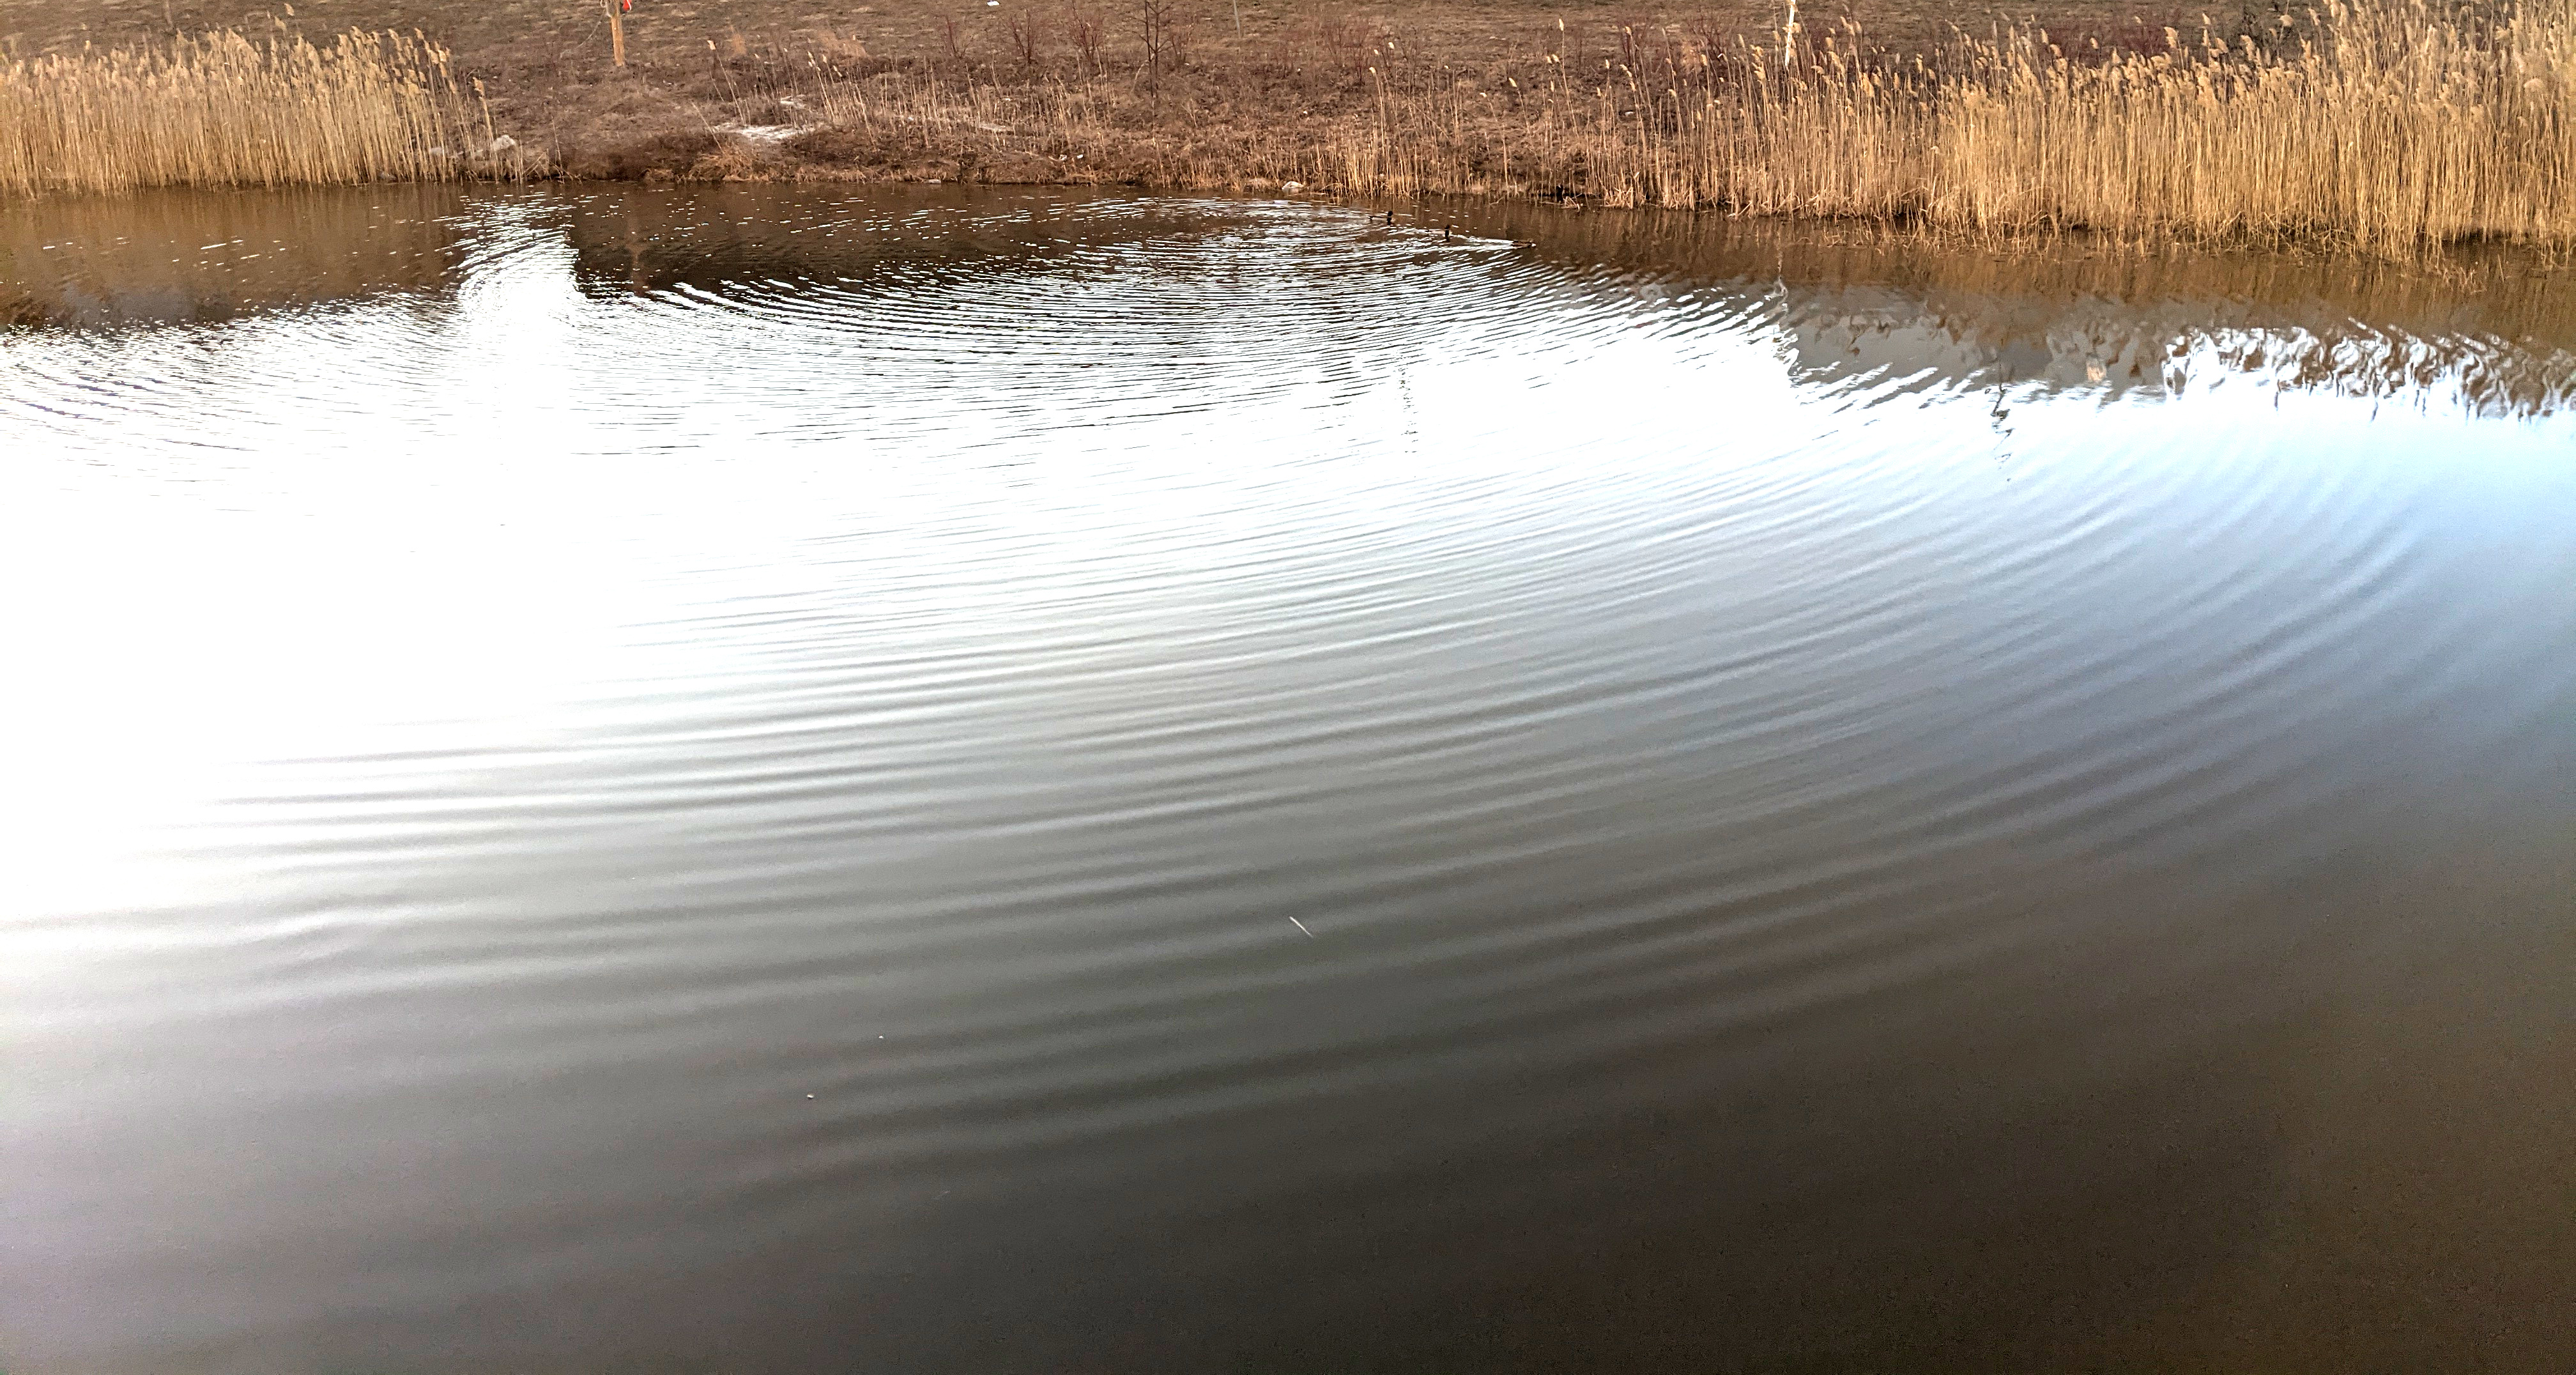
\includegraphics[width=0.9\linewidth]{Figures/Chapter5/fig_pond_waves}
\caption{Small amplitude waves generated by wind on the surface of a small pond on the campus of Ontario Tech University.}
\label{fig_pond}
\end{figure}

These waves are called \emph{gravity waves} since, as we'll see, the main force determining their behaviour is gravity.  However, in some cases -- typically when the wavelengths are very short -- \emph{surface tension} can be the dominant force in attempting to restore equilibrium to the surface.  In that case the waves can behave very differently, and often both forces must be considered.

To begin our discussion, consider a generic example of a surface wave as shown in Figure \ref{fig_generic_wave}.  The shape of the surface -- the interface between the two fluids -- will be described by the function $\eta(x, t)$, so that the surface itself is given by the equation
\begin{equation}
y = \eta(x, t).
\end{equation}
Note that we're setting the direction of gravity to be downward along the negative $y$ direction, in which case $\vec{g} = [0, -g, 0]$ in this coordinate system.

\begin{figure}
\centering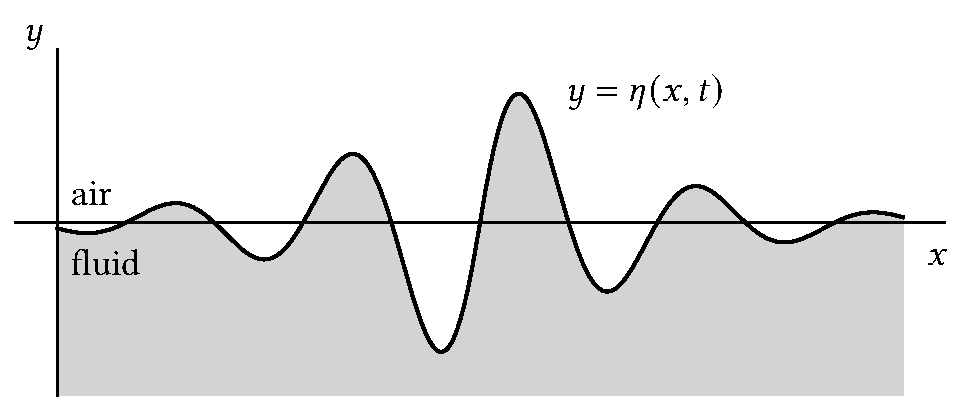
\includegraphics[width=0.8\linewidth]{Figures/Chapter5/fig_generic_wave}
\caption{The surface of a wave is described by the function $\eta(x, t)$.}
\label{fig_generic_wave}
\end{figure}

We'll assume that the fluid is two-dimensional, so there will be no $z$ dependence or flow in that direction:
\[
\vec{u} = [u(x, y, t), v(x, y, t), 0].
\]
We'll also take the flow to be irrotational, so that $\curl \vec{u} = \vec{0}$.  In two dimensions, this means
\[
\dfdx{v}{x} - \dfdx{u}{y} = 0.
\]
It might seem like a leap to assume irrotationality, but if we imagine starting with a perfectly static fluid, with no wave at the interface, then the flow is obviously initially irrotational.  But as time goes on, Kelvin's circulation theorem (see Section \ref{sec_circulation}) guarantees that the flow will remain irrotational -- the circulation must remain zero.

Since our flow is irrotational, we're free to describe it with the velocity potential $\varphi(x, y, t)$.  In two dimensions, $\vec{u} = \grad \varphi$ becomes
\begin{equation}
u = \dfdx{\varphi}{x} \quad \text{and} \quad v = \dfdx{\varphi}{y}.
\end{equation}
Finally, we're still dealing with incompressible fluids, which means the velocity potential must satisfy Laplace's equation:
\begin{equation}
\ddfdx{\varphi}{x} + \ddfdx{\varphi}{y} = 0.
\end{equation}
This lays out the guiding equations behind our discussion of waves; all that's left is to determine the boundary conditions.

% 5.1.2 - The Kinematic and Pressure Conditions

\subsection{The Kinematic and Pressure Conditions}
\label{sec_kin_press_cond}

The first boundary condition comes from the fact that any fluid particle at the surface must remain at the surface.  You might be able to visualize this by imagining dyeing the fluid at the surface; as the surface moves up or down, the dyed fluid stays at the surface.  This means that those fluid particles at the surface must follow the vertical motion of the wave.  We can model this mathematically by defining a new function, $F(x, y, t)$, such that
\begin{equation}
F(x, y, t) = y - \eta(x, t).
\end{equation}
Although in general $F$ can take on any value, all fluid particles at the surface have $F =$ constant -- namely, $F(x, y, t) = 0$ there since $y = \eta(x, t)$ defines our surface.

With the function $F$ constant at the surface, we can obviously write
\[
\frac{DF}{Dt} = 0 \quad \text{on} \quad y = \eta(x, t)
\]
or, expanding the material derivative,
\begin{equation}
\label{eq_kin_cond_md}
\dfdx{F}{t} + (\vec{u} \cdot \grad ) F = 0 \quad \text{on} \quad y = \eta(x, t).
\end{equation}
Now,
\[
\dfdx{F}{t} = \frac{\partial}{\partial t} \Bigl( y - \eta(x, t) \Bigr) = -\dfdx{\eta}{t}
\]
and
\[
(\vec{u} \cdot \grad) F = u \dfdx{F}{x} + v\dfdx{F}{y} = -u \dfdx{\eta}{x} + v,
\]
so equation (\ref{eq_kin_cond_md}) becomes
\[
-\dfdx{\eta}{t} - u\dfdx{\eta}{x} + v = 0,
\]
or
\begin{equation}
\label{eq_kin_cond}
\boxed{
\dfdx{\eta}{t} + u\dfdx{\eta}{x} = v \quad \text{on} \quad y = \eta(x, t).
}
\end{equation}
This is called the \emph{kinematic condition} at the surface; it ensures that fluid particles move with the surface wave.

The second boundary condition at the surface follows from considering the pressure in the fluid:  it must be \emph{continuous} across the interface.  Since we're usually assuming air above the fluid, we'll take the pressure at the surface to be atmospheric pressure, $p_0$, which is of course constant along the surface.  

Consider Euler's equation in the form of equation (\ref{eq_euler_bernoulli}),
\[
\frac{\partial \uu}{\partial t} + (\curl \uu ) \times \uu = -\grad \left( \frac{p}{\rho} + \tfrac{1}{2} \uu^2 + \Phi \right).
\]
The second term on the left is zero here, since we have irrotational flow, and we can write $\vec{u} = \grad \varphi$ and then combine the velocity potential with the other terms in the gradient on the right.  That gives us
\[
\grad \left( \dfdx{\varphi}{t} + \frac{p}{\rho} + \frac{1}{2} \vec{u}^2 + \Phi \right) = 0.
\]
Integrating leads to
\begin{equation}
\label{eq_euler_wave}
\dfdx{\varphi}{t} + \frac{p}{\rho} + \frac{1}{2} \vec{u}^2 + \Phi = G(t),
\end{equation}
where $G(t)$ is the integration ``constant'' -- it can still be a function of time.  But we're free to take $G(t)$ to be anything we want, since it will go away once we take the space derivative. So, for reasons we'll see in a second, let's take it to be
\begin{equation}
G(t) = \frac{p_0}{\rho}.
\end{equation}
Note that it's the constant atmospheric pressure $p_0$ in that equation.

Our next step is to evaluate equation (\ref{eq_euler_wave}) at the surface $y = \eta(x, t)$:
\begin{equation}
\label{eq_pressure_surface}
\dfdx{\varphi}{t} + \frac{p_0}{\rho} + \frac{1}{2} \vec{u}^2 + \Phi = \frac{p_0}{\rho} \quad \text{on} \quad y = \eta(x, t).
\end{equation}
Now we see why that choice of $G(t)$ was made, since the pressure terms cancel out.  Writing $\Phi = gy$ and $\vec{u}^2 = u^2 + v^2$, this becomes
\begin{equation}
\label{eq_pressure_cond}
\boxed{
\dfdx{\varphi}{t} +  \frac{1}{2}(u^2 + v^2) + g\eta = 0 \quad \text{on} \quad y = \eta(x, t).
}
\end{equation}
This is the \emph{pressure condition}, the second boundary condition that must be satisfied by the wave surface.  Together with the kinematic condition and Laplace's equation, they make up the theory of surface waves.  Unfortunately, although Laplace's equation is linear, the boundary conditions are not, and this makes them rather difficult to work with.  


% 5.1.3 - Small Amplitude Waves (linearization)

\subsection{Small Amplitude Waves}

If we restrict our investigation to waves that have an amplitude that is small compared to the wavelength (see Figure \ref{fig_small_wave}), we can make some simplifications.  Let's suppose that the fluid velocities $u$ and $v$ are small, and that therefore the surface $\eta$ doesn't deviate too much from $y = 0$.  If that's the case, then we can assume the derivative $\partial \eta / \partial x$ is \emph{also} small, since the slope of the wave won't deviate too much from horizontal.  If any of the terms in equations (\ref{eq_kin_cond}) or (\ref{eq_pressure_cond}) have two or more of these small quantities multiplied together, we'll drop those terms -- in other words, we'll drop anything that is quadratic or higher in smallness.  This is called \emph{linearizing} the boundary conditions.

\begin{figure}
\centering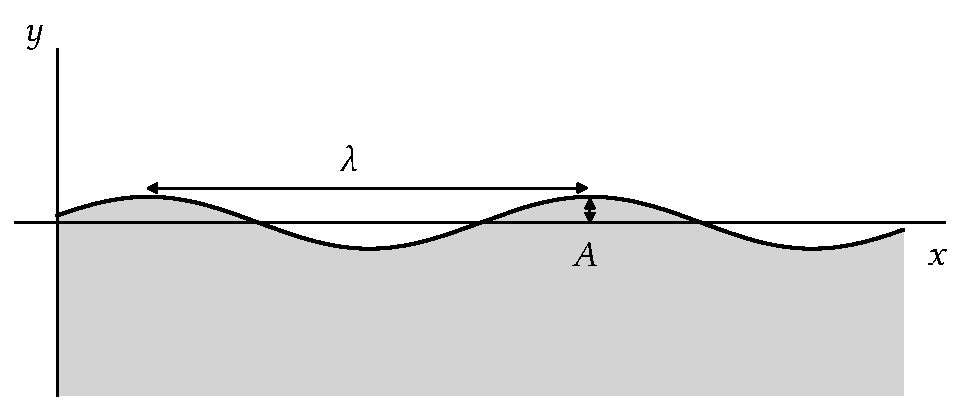
\includegraphics[width=0.8\linewidth]{Figures/Chapter5/fig_small_wave}
\caption{A small-amplitude wave has a wavelength $\lambda \gg A$.}
\label{fig_small_wave}
\end{figure}

Let's start with the kinematic condition, equation (\ref{eq_kin_cond}).  The second term can be dropped since both $u$ and $\partial \eta / \partial x$ are small.  But we can do one other thing, as well.  Let me  write out the condition, being sure to use $y = \eta(x, t)$ in place of $y$:
\[
v(x, \eta, t) = \dfdx{\eta}{t}.
\]
Since $\eta$ is close to zero, we can expand the velocity $v$ about $y = \eta = 0$ in a Taylor expansion, and get
\[
v(x, \eta, t) \approx v(x, 0, t) + \eta \dfdx{v}{y} \bigg|_{\eta=0},
\]
where the higher terms in the expansion were dropped.  In fact, we can drop the second term, as well, since both $\eta$ and $v$ are small, and the kinematic condition becomes
\[
v(x, 0, t) = \dfdx{\eta}{t} \quad \text{on} \quad y=0.
\]
Note that we're now evaluating this at $y=0$, since that's where the surface is to first order. One last thing: we can write this in terms of the velocity potential rather than the velocity using $v = \partial \varphi / \partial y$ and get
\begin{equation}
\label{eq_kin_cond_lin}
\boxed{
\dfdx{\varphi}{y} = \dfdx{\eta}{t} \quad \text{on} \quad y=0.
}
\end{equation}

We can make similar arguments for the pressure condition, equation (\ref{eq_pressure_cond}).  The linearized version is
\begin{equation}
\label{eq_pressure_cond_lin}
\boxed{
\dfdx{\varphi}{t} + g\eta = 0 \quad \text{on} \quad y=0.
}
\end{equation}



% 5.1.4 - Sinusoidal Waves (dispersion relation, potential, example of fluid path under wave)

\subsection{Sinusoidal Waves on Deep Water}

As a simple but important example, suppose the surface can be described by a sinusoidal travelling wave, given by
\begin{equation}
\label{eq_sin_eta}
\eta(x, t) = A \cos(kx - \omega t),
\end{equation}
where $k = 2\pi / \lambda$ is the wave number and $\omega = 2\pi \nu$ is the angular frequency of the wave.

The boundary conditions will not only allow us to find the velocity potential of the fluid, but also will place important restrictions on the behaviour of the waves.  The linearized kinematic condition says
\[
\dfdx{\varphi}{y} = \dfdx{\eta}{t} = \omega A \sin(kx - \omega t),
\]
suggesting that the potential takes the form
\begin{equation}
\label{eq_pot_suggestion}
\varphi(x, y, t) \propto f(y) \sin (kx - \omega t).
\end{equation}
We can find the unknown function $f(y)$ by ensuring that the potential satisfies Laplace's equation,
\[
\ddfdx{\varphi}{x} + \ddfdx{\varphi}{y} = 0.
\]
Substituting equation (\ref{eq_pot_suggestion}) into Laplace's equation leads to 
\[
-k^2 f(y) \sin (kx - \omega t) + f''(y) \sin (kx - \omega t) = 0.
\]
Cancelling out the sine term and rearranging gives the familiar differential equation
\[
f'' = k^2 f,
\]
with general solution
\[
f(y) = C e^{ky} + D e^{-ky}.
\]

Although we've discussed at length the boundary conditions at the surface of the fluid, we haven't mentioned what happens as we go down in depth.  Two options are possible:  that the fluid extends to infinity below the surface (these waves are called \emph{deep water waves}) or that a ``floor'' exists at some depth $y = -h$.  We'll use the first possibility here, and you can explore the effects of finite depth in Problem \ref{prob_finite_depth}.

If the fluid extends down to $y \to -\infty$, then we have to drop the second term of our solution by setting $D = 0$ -- otherwise the potential will blow up as we go deeper into the fluid.  We have, therefore, 
\[
\varphi(x, y, t) = C e^{ky} \sin (kx - \omega t).
\]
We can find the constant $C$ by using the kinematic pressure condition, equation (\ref{eq_kin_cond_lin}); taking the derivatives and setting $y = 0$ gives
\[
kC \sin(kx - \omega t) = \omega A \sin (kx - \omega t),
\]
or
\begin{equation}
kC = \omega A.
\end{equation}
Thus, the velocity potential is
\begin{equation}
\label{eq_sin_pot}
\varphi(x, y, t) = \frac{\omega A}{k} e^{ky} \sin (kx - \omega t).
\end{equation}
This holds \emph{everywhere} in the fluid, not just at the surface, and we can use it to explore the motion of the fluid below the waves -- we'll do that in a moment.  But first, what about the pressure condition?  We haven't applied that yet.

Evaluating the pressure condition, equation (\ref{eq_pressure_cond_lin}), gives
\[
-\frac{\omega^2}{k} \cos(kx - \omega t) + gA \cos(kx - \omega t) = 0,
\]
or
\begin{equation}
\label{eq_disp_relation}
\boxed{
\omega^2 = gk.
}
\end{equation}
This is an important relationship between the frequency of a wave and its wavelength, and is called the \emph{dispersion relation} for deep water gravity waves.  You might be more familiar with \emph{disperionless} waves like waves on a string or even electromagnetic waves.  In these kinds of waves, $\omega \propto k$.  Because sinusoidal waves travel with speed
\begin{equation}
c = \frac{\omega}{k},
\end{equation}
the speed of the wave won't depend on the wavelength.  But for water waves, with $\omega \propto \sqrt{k}$, different wavelengths will travel at different speeds, since
\[
c = \sqrt{\frac{g}{k}} = \sqrt{\frac{g\lambda}{2\pi}}.
\]
Thus, longer wavelengths will travel \emph{faster} than shorter ones.  This leads to some interesting surface wave effects, one of which is shown in Figure \ref{fig_gravity_ripples} -- the waves with longer wavelengths will travel further from the source of the disturbance in the pond, giving the ripples a distinctive look.

\begin{figure}
\centering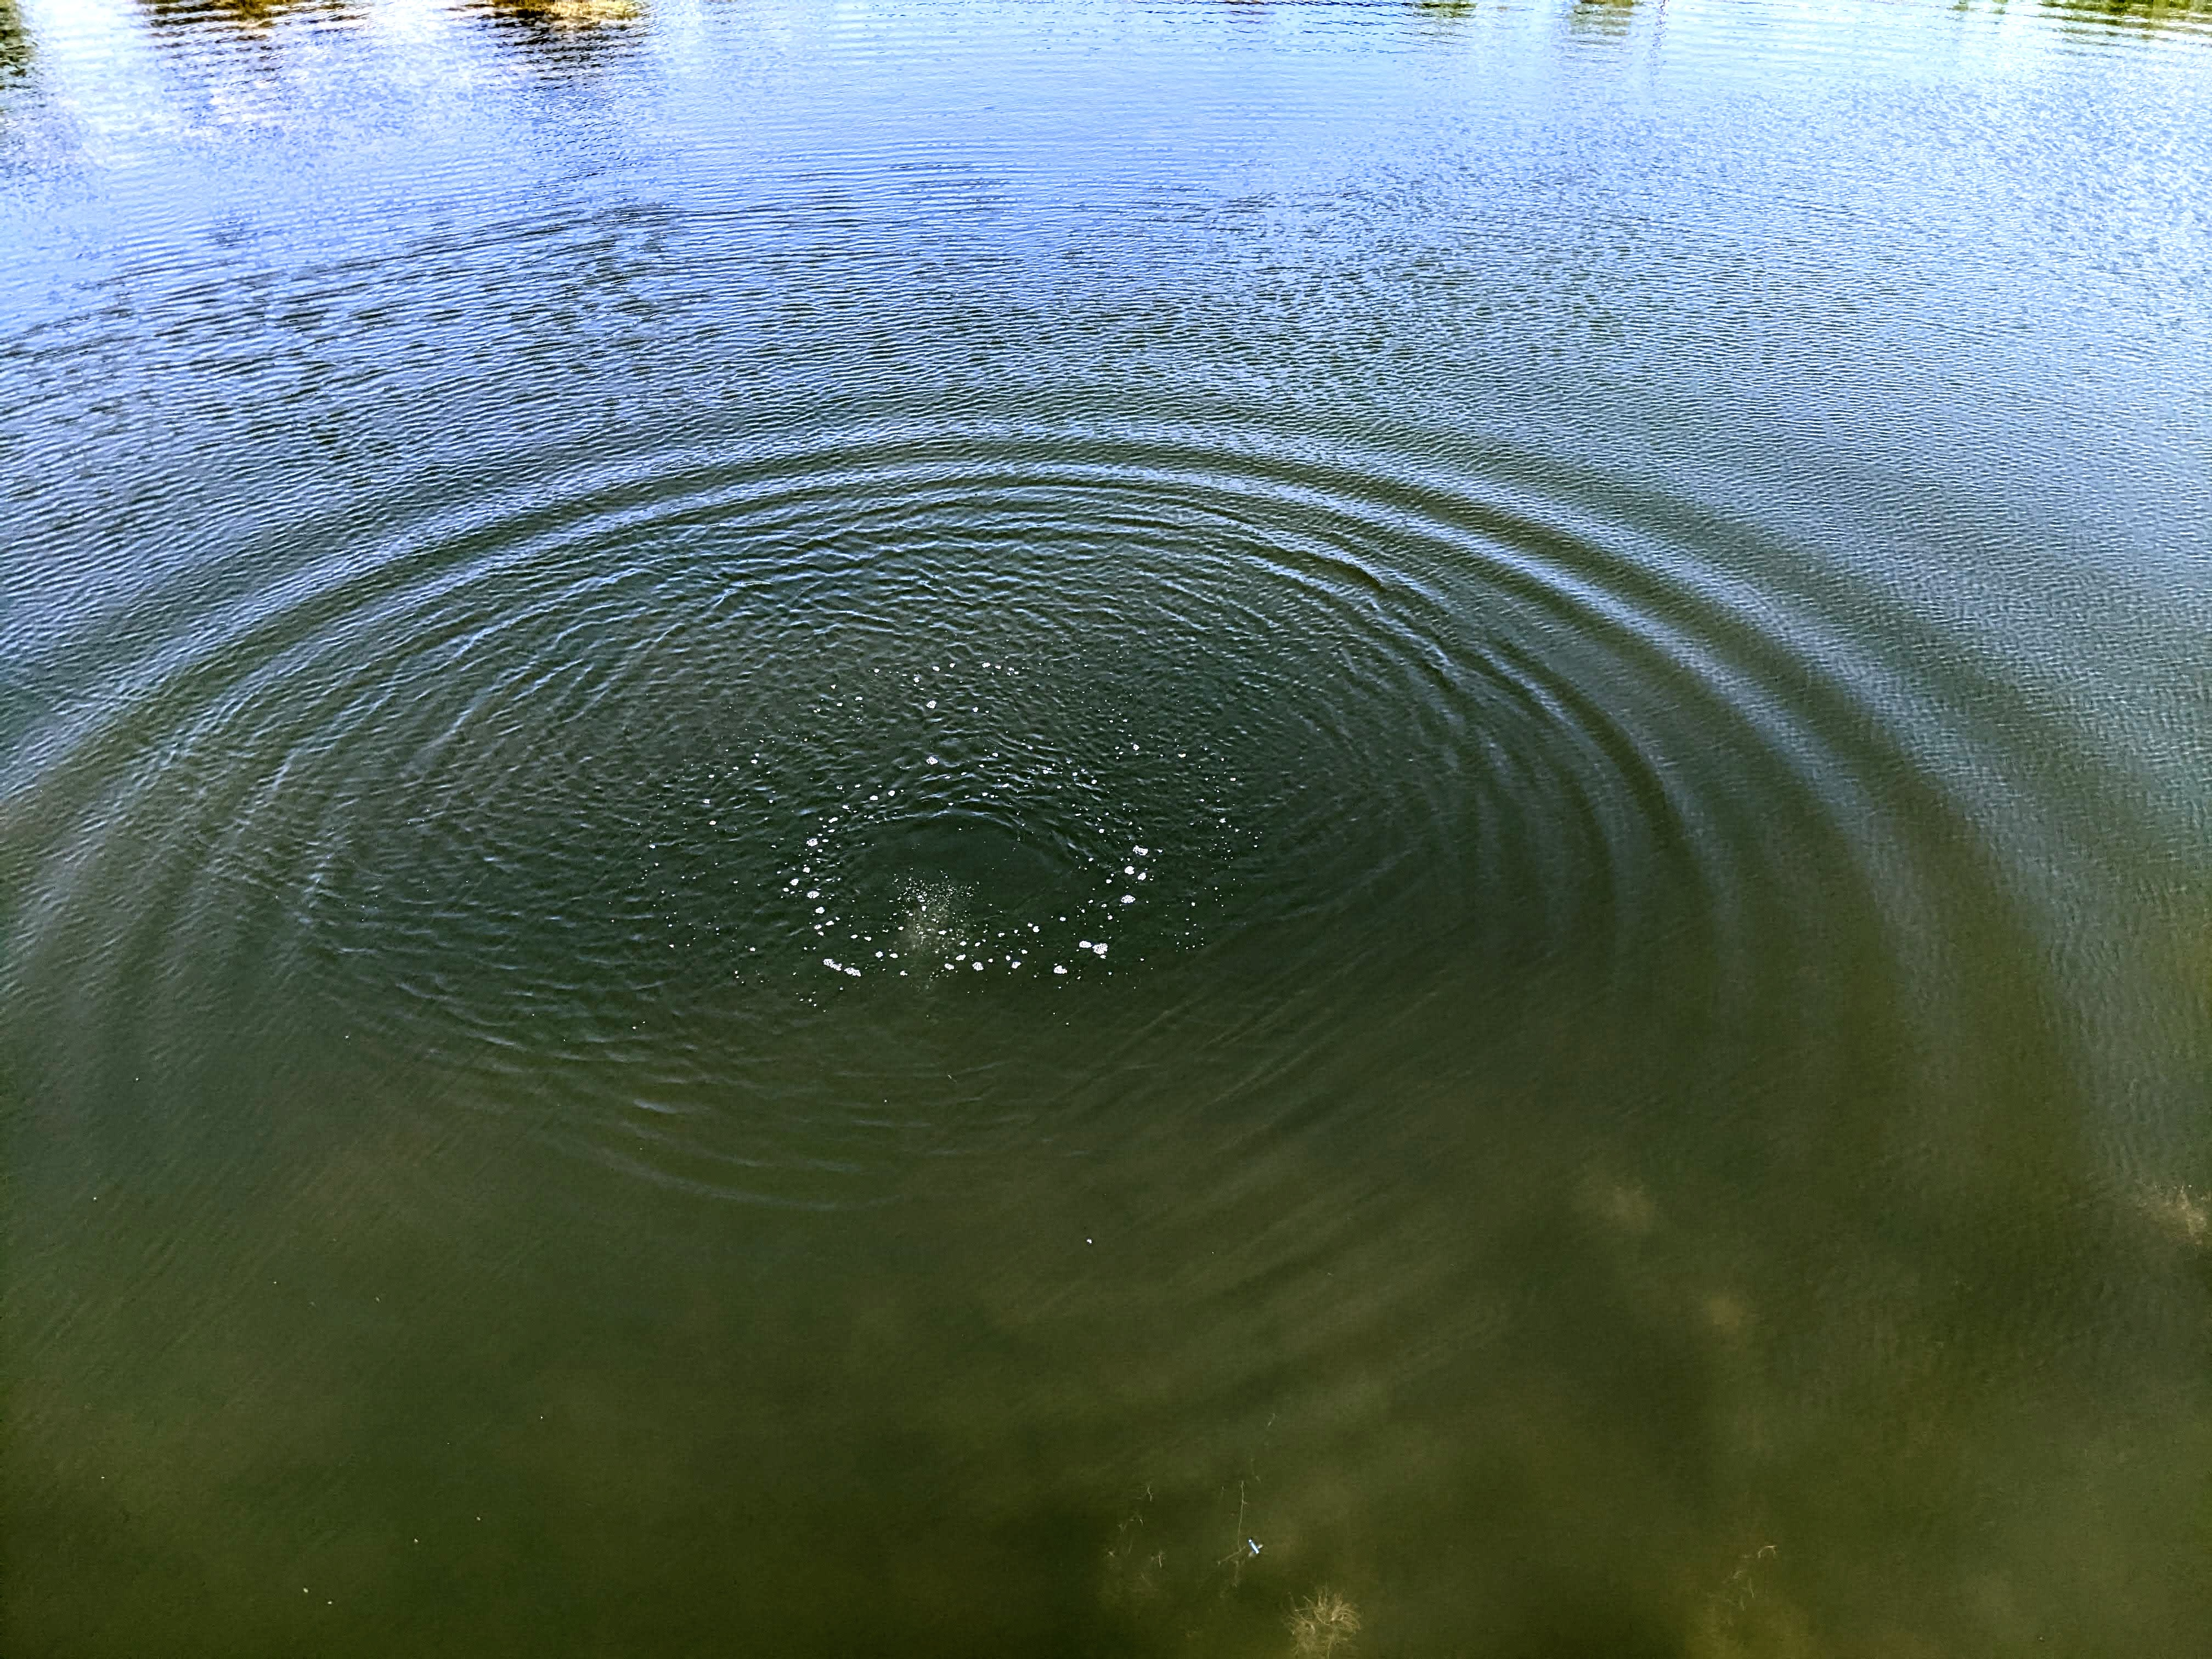
\includegraphics[width=0.8\linewidth]{Figures/Chapter5/fig_gravity_ripples}
\caption{A disturbance (from dropping a large stone) on the surface of a pond creates gravity waves which propagate outward.  As you can see in the photograph, the largest wavelengths move fastest and thus travel furthest.}
\label{fig_gravity_ripples}
\end{figure}

\begin{example}[Fluid motion under the surface]

Now that we have the velocity potential $\varphi(x, y, t)$, we can examine the entire fluid flow.  In particular, imagine a single fluid particle initially at some depth under the surface.  What path does the particle take as the surface waves propagate to the right?

Start with the fluid velocity, which we find from the potential:
\[
u = \dfdx{\varphi}{x} = A \omega e^{ky} \cos (kx - \omega t),
\]
and
\[
v = \dfdx{\varphi}{y} = A \omega e^{ky} \sin (kx - \omega t).
\]
Fluid particles, of course, follow the fluid, so we can write the change in position of a particular fluid particle as
\[
\frac{dx}{dt} = u \quad \text{and} \quad \frac{dy}{dt} = y.
\]
This gives us two coupled differential equations to solve.  But we can uncouple them by making a reasonable assumption:  that the fluid particle doesn't deviate too much from its \emph{mean position} $(\bar{x}, \bar{y})$.  That is, 
\[
x = \bar{x} + x'  \quad \text{and} \quad y = \bar{y} + y',
\]
where $x'$ and $y'$ are small.

Since $\bar{x}$ and $\bar{y}$ are constant, we can write
\[
\frac{dx}{dt} = \frac{dx'}{dt} = u \approx A \omega e^{k\bar{y}} \cos (k \bar{x} - \omega t)
\]
and 
\[
\frac{dy}{dt} = \frac{dy'}{dt} = v \approx A \omega e^{k\bar{y}} \sin (k \bar{x} - \omega t).
\]
Note that now the right-hand-sides contain only the (constant) mean positions, meaning that we can simply integrate to find the particle path and get
\begin{equation}
x' = -A e^{k\bar{y}} \sin(k\bar{x} - \omega t), \quad  y' = A e^{k\bar{y}} \cos (k\bar{x} - \omega t).
\end{equation}
As time goes on and the surface wave travels horizontally, the fluid particles under the surface trace out \emph{circles} of radius $Ae^{k\bar{y}}$.  As the depth increases, the circles get smaller, as shown in Figure \ref{fig_circle_paths}.

\end{example}


\begin{figure}
\centering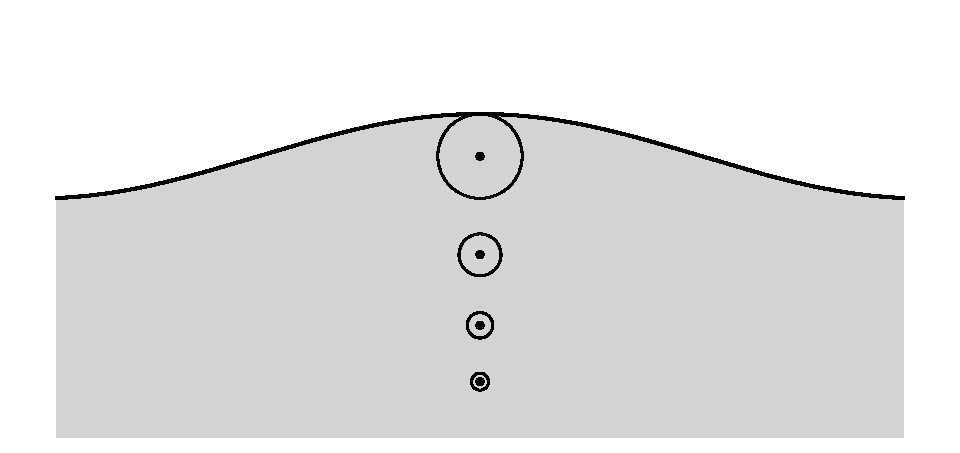
\includegraphics[width=0.8\linewidth]{Figures/Chapter5/fig_circle_paths}
\caption{Fluid particles in deep water under surface waves move in circular paths about their mean position (the dot) with radii that get exponentially smaller with decreasing depth.  If the wave is propagating to the right, the paths will be clockwise.}
\label{fig_circle_paths}
\end{figure}

% 5.1.5 - Capillary Waves (surface tension effects, new BCs, surface tension-dominated waves, etc; include pic of the two types of waves, plus downstream/upstream stuff and pic of that)


\subsection{Capillary Waves}

In Section \ref{sec_kin_press_cond} we took the pressure to be continuous across the fluid-air interface, so that the pressure at the surface of the fluid was atmospheric pressure $p_0$.  However, this isn't quite true -- if the surface is \emph{curved}, as ours of course will be, then there is a small pressure discontinuity across the surface due to the \emph{surface tension} of the fluid.  Surface tension is related to the cohesion of fluid molecules and results in a force (per unit length) that is tangential to the surface of the fluid.  Water, for example, has a surface tension of $T = 72.8$ mN/m at a temperature of 20 C.  

This tangential force will change the surface boundary conditions we just derived, although in many cases the effect can be neglected and gravity waves are a good approximation.  However, for small disturbances to the surface or short wavelengths, surface tension can have a noticeable and interesting effect.  In cases where surface tension is the dominant force, the waves are called \emph{capillary waves}, and where both gravity and surface tension are important the waves generated are sometimes called \emph{gravity-capillary waves}.

\begin{figure}
\centering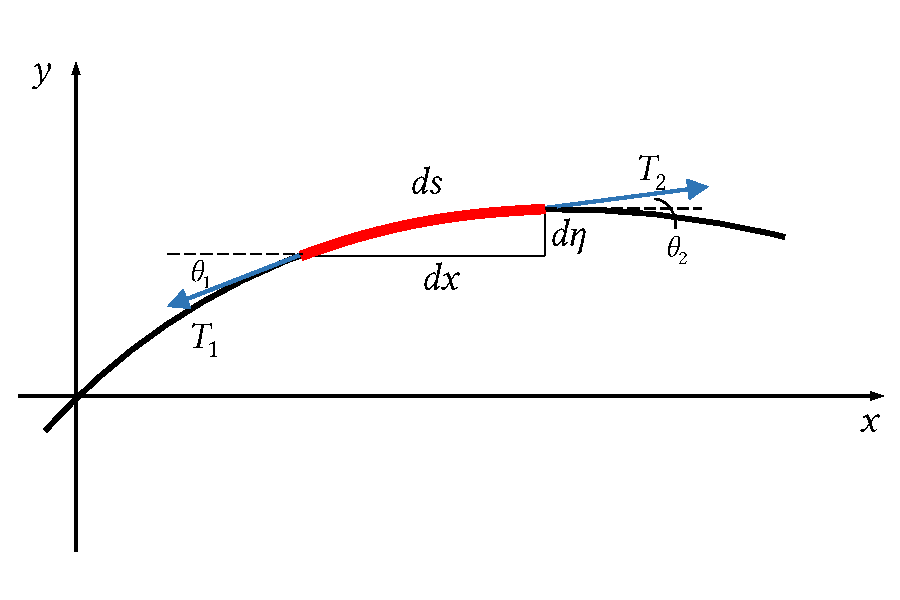
\includegraphics[width=0.8\linewidth]{Figures/Chapter5/fig_surface_tension}
\caption{Surface tension creates a force tangential to the surface of the fluid.}
\label{fig_surface_tension}
\end{figure}

We can derive the pressure discontinuity across the surface by considering a small element of the fluid $ds$ as shown in Figure \ref{fig_surface_tension}.  Remember that although we're treating $ds$ as a line element, our fluid is two-dimensional and so $ds$ is actually an infinitesimally thin strip of area along the face of the wave.  Surface tension exerts a force at either end of $ds$ ($T_1$ on the left side and  $T_2$ on the right), and it's this difference we want to calculate.  Since we're still assuming small amplitude waves only, we can take the slope $d\eta/dx$ to be small.  This has a number of consequences:
\begin{itemize}
\item The angles $\theta_1$ and $\theta_2$ are small, and we can use small-angle approximations for sine and cosine, dropping any terms quadratic or higher in $\theta$.
\item The fluid element executes \emph{vertical} motion only -- it goes up and down but not side-to-side.  This means that there should be no net force in the horizontal ($x$) direciton.
\item We can take $ds = \sqrt{dx^2 + d\eta^2} \approx dx$.
\end{itemize}

Examining the horizontal components of the tensions, we see that
\[
T_{2x} - T_{1x} = T_2 \cos\theta_2 - T_1 \cos \theta_1 \approx T_2 - T_1.
\]
But because there is no net force in this direction, we must have $T_2 = T_1$. Since the magnitudes of the two surface tensions are the same, I'll just call it $T$.

In the vertical direction, we have
\[
T_{2y} - T_{1y} = T_2 \sin\theta_2 - T_1 \sin \theta_1 = T ( \theta_2 - \theta_1),
\]
but we can write the angles in terms of the slopes as
\[
\theta_2 \approx \frac{\partial\eta}{\partial x}\bigg|_{x + dx} \quad \text{and} \quad \theta_1 \approx \frac{\partial\eta}{\partial x}\bigg|_{x - dx}
\]
where $x$ is the location of the fluid element we're considering.  The difference in the vertical surface tensions is therefore
\begin{equation}
T_{2y} - T_{1y} = T \left( \frac{\partial\eta}{\partial x}\bigg|_{x+dx} - \frac{\partial\eta}{\partial x} \bigg|_{x-dx} \right) = T \ddfdx{\eta}{x} \, dx,
\end{equation}
where the \emph{second} derivative comes from the difference of two \emph{first} derivatives.

Now, the quantity $T \partial^2\eta / \partial x^2$ is the net force on the fluid per unit \emph{area} -- it's a pressure.  This pressure must be balanced by the difference in pressure above (atmospheric pressure $p_0$) and below ($p$) the surface, so 
\begin{equation}
p_0 - p = T \ddfdx{\eta}{x} \quad \text{at} \quad y = \eta(x, t).
\end{equation}
If the surface is concave up, then the second derivative is positive, and the pressure just above the fluid is greater than the pressure just below the surface.  If the surface is concave down, the opposite happens:  pressure is greater just below the surface.

We can incorporate this pressure difference into our pressure condition by repeating the steps in Section \ref{sec_kin_press_cond}; when we get to equation (\ref{eq_pressure_surface}), we need to use the new pressure at the surface, 
\[
p = p_0 - T \ddfdx{\eta}{x},
\]
in place of just the atmospheric pressure $p_0$.  That just adds an extra term in the pressure condition, which becomes
\begin{equation}
\label{eq_pressure_cond_cap}
\dfdx{\varphi}{t} +  \frac{1}{2}(u^2 + v^2) + g\eta  - \frac{T}{\rho} \ddfdx{\eta}{x} = 0 \quad \text{on} \quad y = \eta(x, t).
\end{equation}
Linearizing as we did previously gives
\begin{equation}
\label{eq_pressure_cond_cap_lin}
\boxed{
\dfdx{\varphi}{t} + g\eta - \frac{T}{\rho} \ddfdx{\eta}{x} = \quad \text{on} \quad y=0.
}
\end{equation}

With a new boundary condition, the dispersion relation we found for sinusoidal waves, equation (\ref{eq_disp_relation}), will be modified as well.  As you can show in Problem \ref{prob_grav_cap_dispersion}, the new dispersion relation for gravity-capillary waves is given by
\begin{equation}
\boxed{
\omega^2 = gk + \frac{Tk^3}{\rho}.
}
\end{equation}
The speed of a sinusoidal travelling wave can be found as usual from $c = \omega/k$, and is
\begin{equation}
c = \sqrt{ \frac{g}{k} + \frac{Tk}{\rho} }.
\end{equation}

Consider the dimensionless parameter $\tau$, defined as
\begin{equation}
\tau = \frac{Tk^2}{\rho g},
\end{equation}
which acts as a measure of the relative strength of the surface tension and gravity forces; notice, though, that $\tau$ also depends on wavelength through $k$, a point we'll return to in a moment.  When $\tau \gg 1$, surface tension is the dominant force and the waves are capillary, which travel at a speed
\begin{equation}
c = \sqrt{\frac{Tk}{\rho}} = \sqrt{ \frac{2\pi T}{\rho \lambda}}.
\end{equation}
For these waves, longer wavelengths actually travel \emph{slower}, in contrast to gravity waves where the opposite is true.  This is evident in a comparison between Figure \ref{fig_gravity_ripples}, which shows circular gravity waves generated by a disturbance, and Figure \ref{fig_cap_ripples}, which show circular capillary waves -- much smaller in wavelength and created by a smaller disturbance.  


\begin{figure}
\centering\includegraphics[width=0.9\linewidth]{Figures/Chapter5/fig_cap_ripples}
\caption{Capillary waves created by dropping a tiny pebble into water.  Notice that the shorter wavelengths have travelled further than the longer ones.}
\label{fig_cap_ripples}
\end{figure}


\begin{figure}
\centering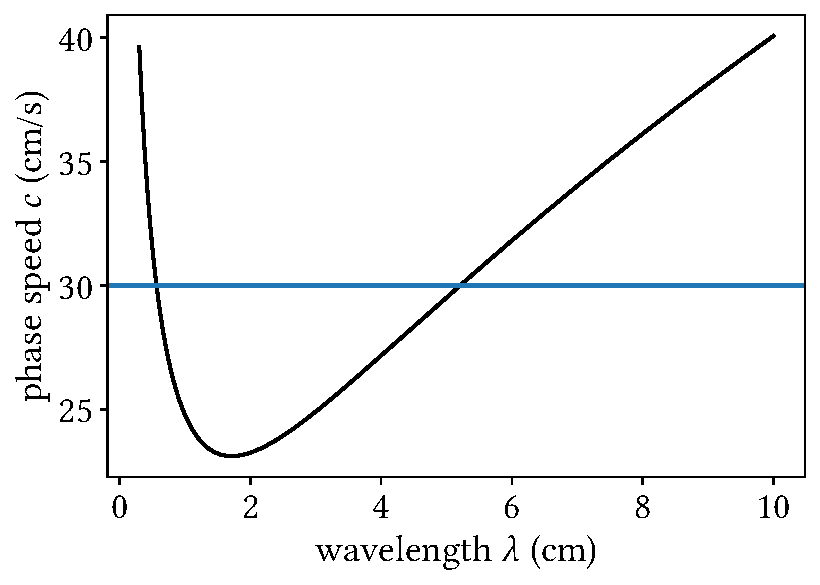
\includegraphics[width=0.7\linewidth]{Figures/Chapter5/fig_grav_and_cap}
\caption{Wave speed $c$ versus wavelength of water waves.}
\label{fig_grav_and_cap}
\end{figure}


Keep in mind, however, that both gravity and capillary waves can be present in a general disturbance depending on the wavelength of the sinusoidal wave.  For water, for example, waves with a wavelength of $\lambda \sim 1.7$ cm have $\tau \sim 1$.  Waves with wavelengths longer than this have $\tau \ll 1$, so gravity waves will dominate, and waves with $\lambda > 1.7$ cm will have $\tau \gg 1$ and capillary waves will dominate.  Consider Figure \ref{fig_grav_and_cap}, which plots the wave speed $c$ as a function of wavelength $\lambda$ (using water for values of $\rho$ and $T$).  There is a \emph{minimum} speed at
\[
k = \sqrt{\frac{\rho g}{T}},
\]
corresponding to $\lambda = 1.7$ cm for water, which is
\begin{equation}
c_\text{min} = \left( \frac{4gT}{\rho} \right)^{1/4},
\end{equation}
or about 23 cm/s for water.  What does this mean?  Consider water streaming past an obstacle with speed $U$; Figure \ref{fig_stream_obstacle} shows a thin pole in a creek.  If $U < c_\text{min}$, there will be \emph{no} steady waves generated, and if $U > c_\text{min}$, there will be \emph{two} kinds of waves generated, since two different wavelengths can produce the same wave speed, as the horizontal line in Figure \ref{fig_grav_and_cap} shows.  For reasons that we'll see in the next section, gravity waves move downstream, but the capillary waves generated by the obstacle will actually move upstream, giving the water the unique ``folding'' effect seen in Figure \ref{fig_stream_obstacle}.

\begin{figure}
\centering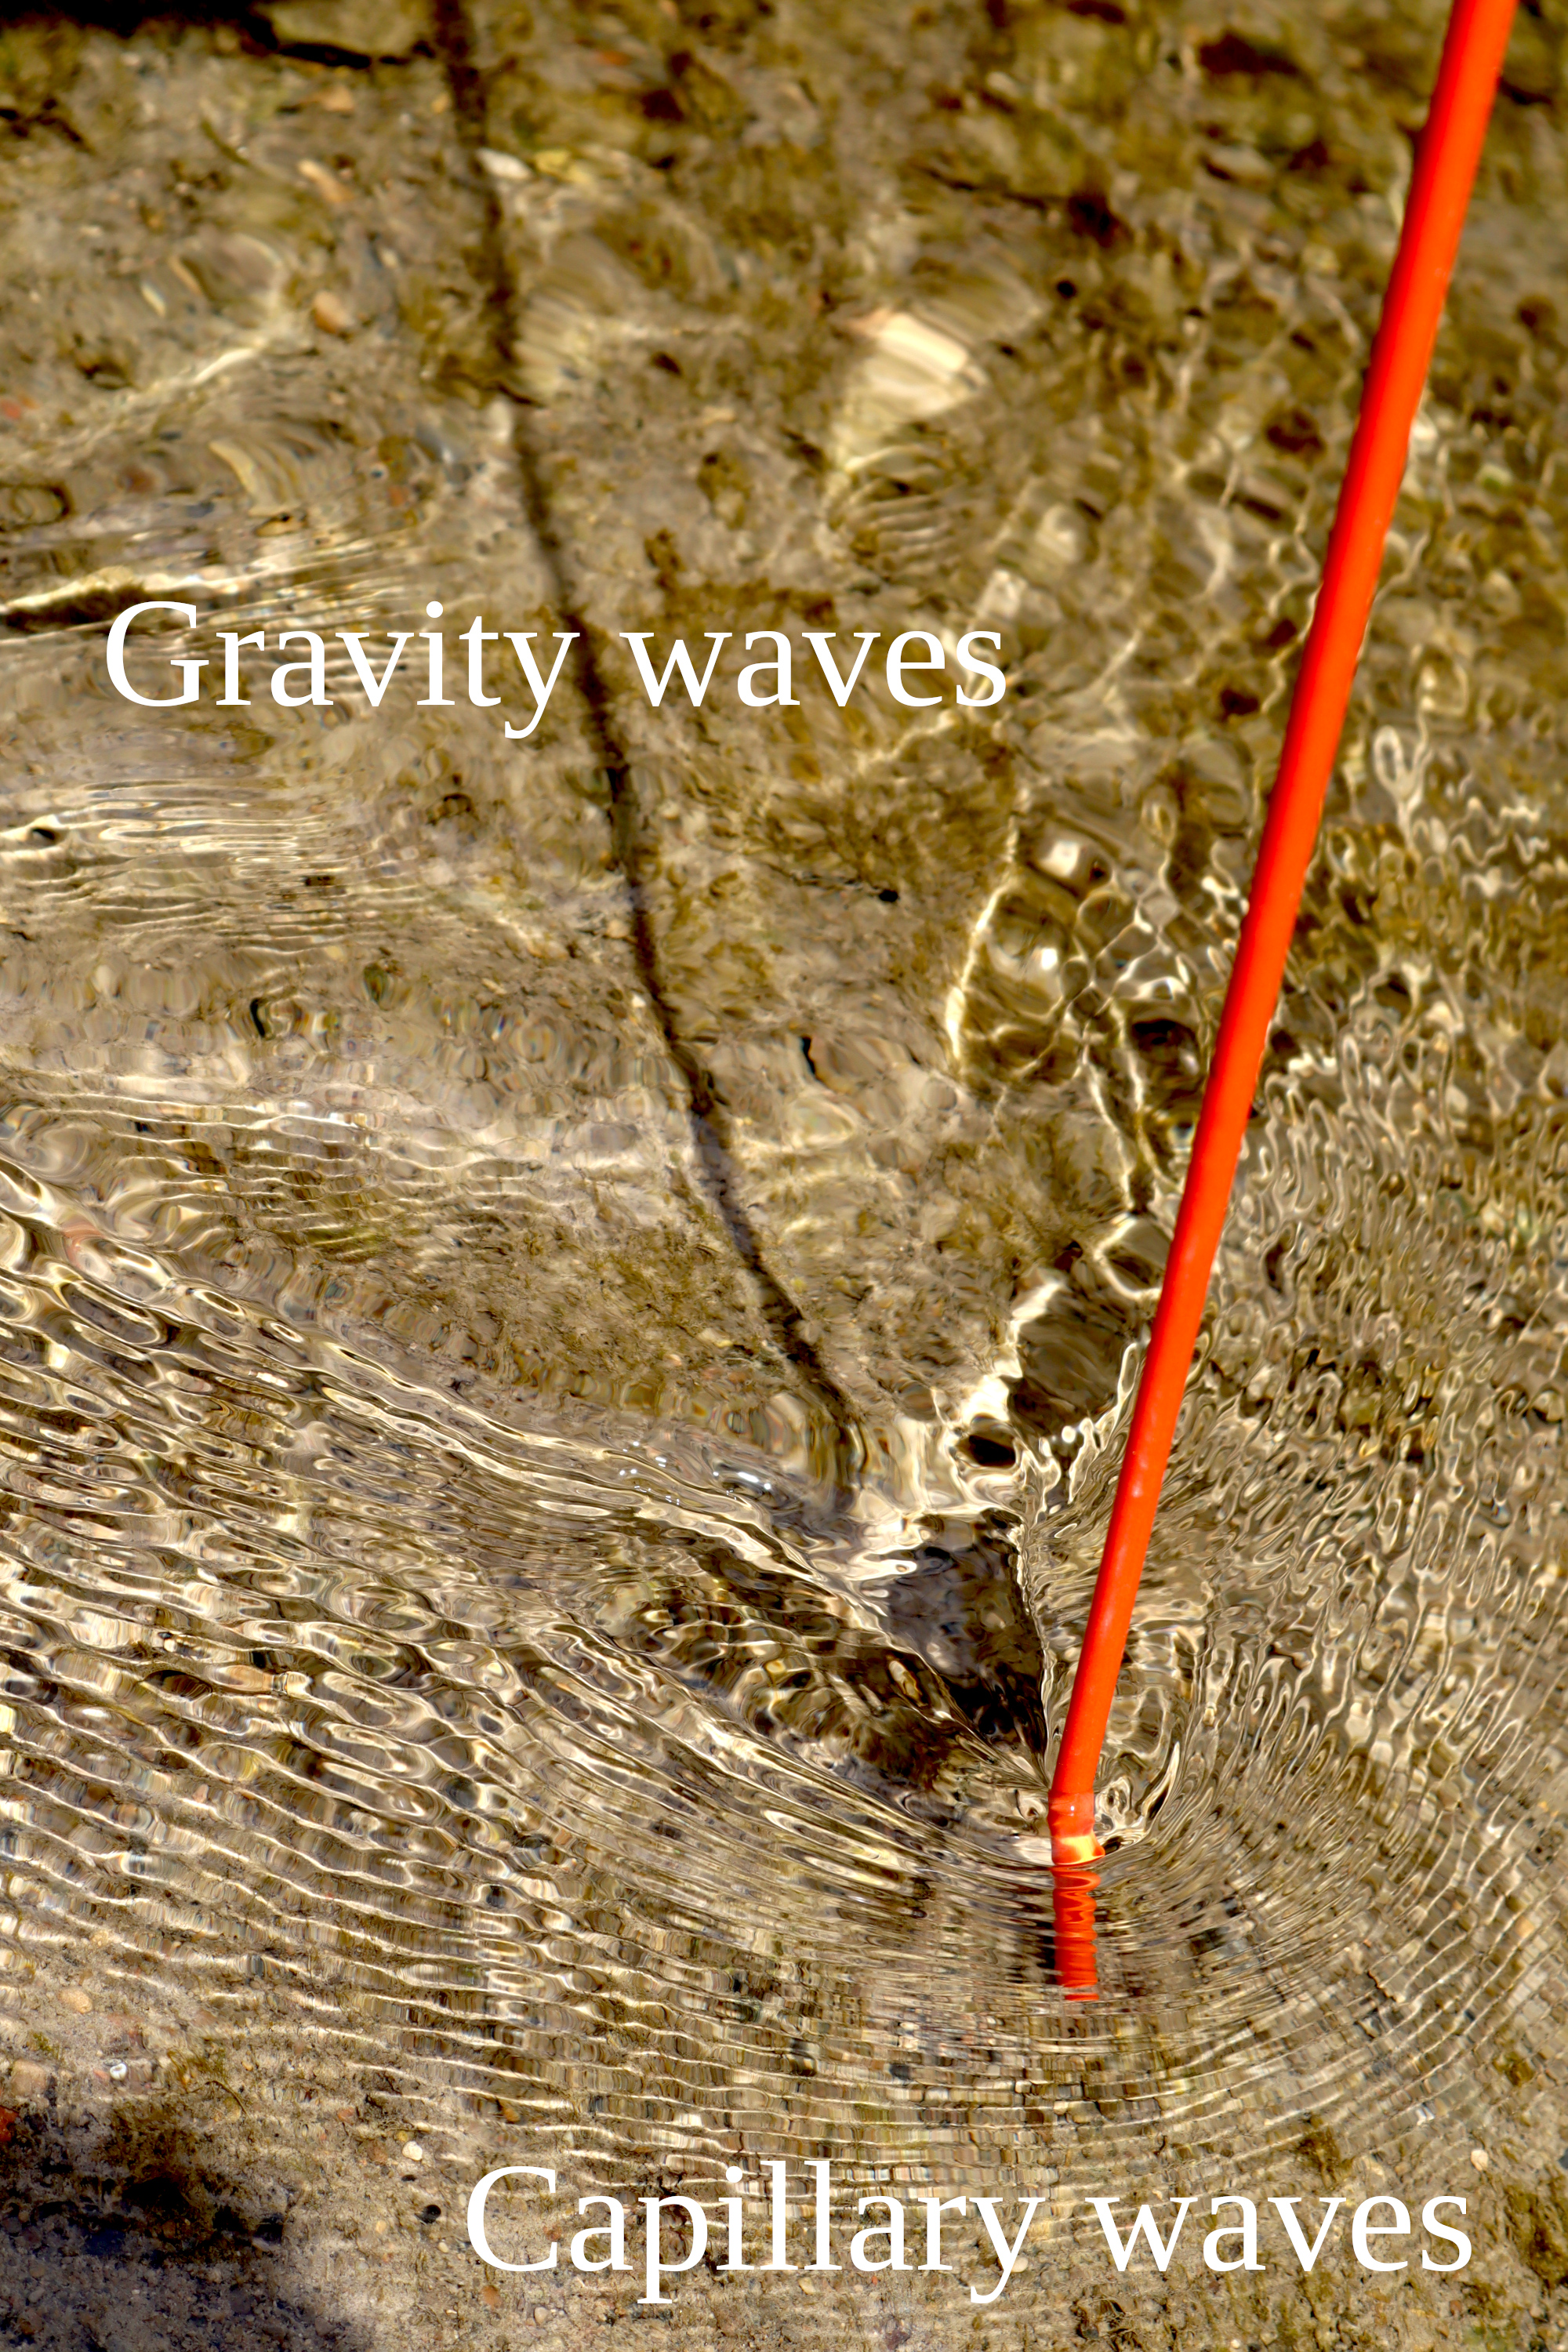
\includegraphics[width=0.6\linewidth]{Figures/Chapter5/fig_stream_obstacle}
\caption{The East Oshawa Creek flows past an obstacle at a speed sufficient to produce both capillary waves (upstream) and gravity waves (downstream; they're a little harder to see because of the much longer wavelength).}
\label{fig_stream_obstacle}
\end{figure}


%
%  SECTION 5.2 - Group Waves
%

\section{Non-Sinusoidal Waves}

% 5.2.1 - Fourier stuff

\subsection{Fourier Series}

Although sinusoidal waves are both simple and important, there are situations where a generated wave is decidedly \emph{not} sinusoidal.  However, even in cases where the wave shape is complicated, the theory of Fourier analysis allows us to represent that shape as a series of sines and cosines.  Perhaps a quick review of Fourier series and transforms is in order.\footnote{For more detail on Fourier analysis, see \emph{Mathematical Methods for Physicists}, 4th edition, by Arfken  and Weber, chapters 14 and 15.}

Any \emph{periodic} function $f(x)$ can be written as a series of sines and cosines,
\[
f(x) = \frac{a_0}{2} + \sum_{n=1}^{\infty} a_n \cos(nx) +  \sum_{n=1}^{\infty} b_n \sin(nx),
\]
or, more conveniently, as exponentials,
\begin{equation}
\label{eq_fourier_series}
f(x) = \sum_{n=1}^\infty c_n e^{inx}.
\end{equation}
Now, for a surface wave, we'll need to include \emph{time} as well, but that's simple enough to do; in general, we can write a travelling surface wave as
\begin{equation}
\label{eq_fourier_waves}
\eta(x, t) = \sum_{n=1}^\infty A_n e^{i(k_n x - \omega_n t)},
\end{equation}
where $k_n$ and $\omega_n$ are the wave number and frequency of the $n$th wave.

\begin{figure}
\centering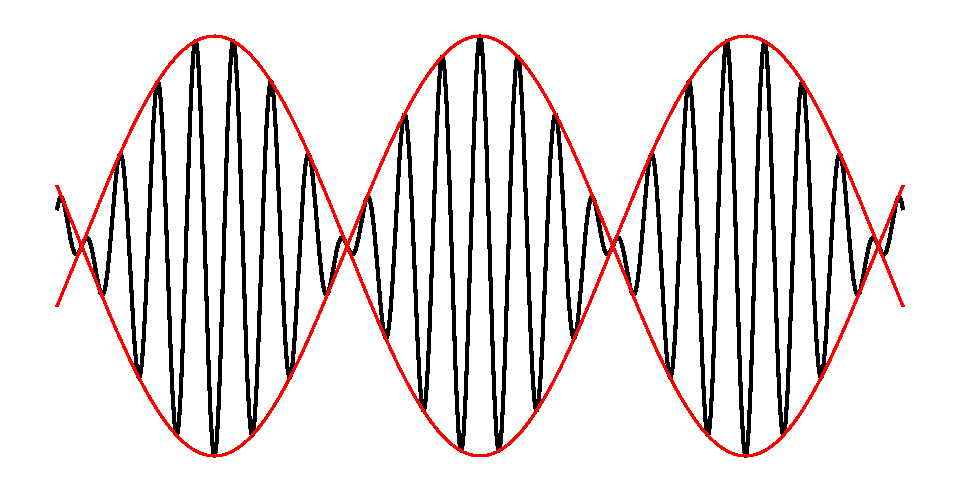
\includegraphics[width=0.8\linewidth]{Figures/Chapter5/fig_two_cosines}
\caption{A surface wave formed by the addition of two cosine waves with similar wavenumber.}
\label{fig_two_cosines}
\end{figure}

\begin{example}[Two cosines]
Let's try a simple example and consider a travelling wave comprised of two cosines of equal amplitude,
\begin{equation}
\label{eq_two_cosines}
\eta(x, t) = A \cos(k_1 x - \omega_1 t) + A \cos(k_2 x - \omega_2 t),
\end{equation}
and further suppose that the wave numbers $k_1$ and $k_2$ are similar, so that we can write
\[
k_1 = k - \Delta k \quad \text{and} \quad k_2 = k + \Delta k.
\]
We'll assume the same for the frequencies $\omega_1$ and $\omega_2$ as well:
\[
\omega_1 = \omega - \Delta \omega \quad \text{and} \quad \omega_2 = \omega + \Delta \omega.
\]
If we substitute these expressions into equation (\ref{eq_two_cosines}), we can write the shape of the wave as (see Problem \ref{prob_two_cosines})
\begin{equation}
\label{eq_two_cosines_ans}
\eta(x, t) = 2A \cos(\Delta k \, x - \Delta \omega \, t) \cos(kx - \omega t).
\end{equation}
This is just the equation of a single sinusoidal wave travelling with speed $c = \omega/k$, but the amplitude of this sinusoidal wave is \emph{modulated} by the term in front, sometimes called the \emph{envelope}.  This is shown in Figure \ref{fig_two_cosines}, with the envelope shown in red.
\end{example}



We've seen, then, that it's possible to represent more complicated wave shapes by adding together sinusoidal waves.  However, a Fourier series like this will also be \emph{periodic}, which is not always the case in nature -- think of a single disturbance in a body of water generating a wave.  To describe a \emph{wave packet} like this, we need to instead use a Fourier integral.

% 5.2.2 - Wave Packets

\subsection{Wave Packets}

The Fourier integral is the generalization of the Fourier series (equation \ref{eq_fourier_series}) by letting the indexed parameter $n$ becomes a continuous parameter $k$.  In that case the sum becomes an integral, and any function (including non-periodic ones) can be written as
\begin{equation}
f(x) = \frac{1}{\sqrt{2\pi}} \int_{-\infty}^{\infty} a(k) e^{ikx} \, dk.
\end{equation}
Here $a(k)$ (which is a complex function even if $f(x)$ is real) is called the \emph{Fourier transform} of the function $f(x)$, and can be calculated by 
\[
a(k) = \frac{1}{\sqrt{2\pi}} \int_{-\infty}^{\infty} f(x) e^{-ikx} \, dx.
\]

\begin{figure}
\centering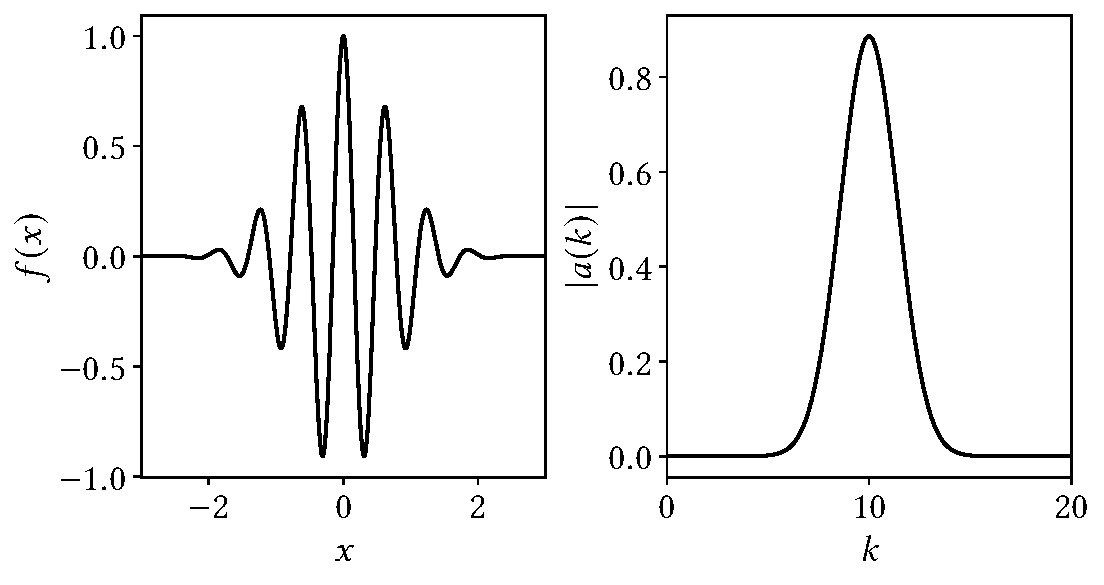
\includegraphics[width=0.8\linewidth]{Figures/Chapter5/fig_fourier_example}
\caption{The Fourier transform of a simple wave packet.  The transform $a(k)$ shows that most of the spectrum consists of wave numbers near $k_0 = 10$.}
\label{fig_fourier_example}
\end{figure}

As an example, consider the function
\[
f(x) = \cos(k_0 x) e^{-x^2},
\]
shown in the left panel of Figure \ref{fig_fourier_example}.  In the plot, I've set $k_0 = 10$.  This is a classic ``wave packet'' shape, and is not periodic.  We'll explore surface waves that look like this in a moment; the key feature we'll use is shown in the right hand panel, which is the Fourier transform $a(k)$ (actually, it's the absolute value $|a(k)|$ since it's a complex function).  Imagine the original function $f(x)$ consisting of a series of sinusoidal waves, like we did above, except this time the index is continuous -- hence the integral instead of the summation.  The Fourier transform of the wave packet tells us the wave numbers of those sinusoidal waves; in this case we see that most of the waves have a wave number close to $k_0 = 10$, but that's not the only wave number involved.  In fact, to make up this wave packet shape, we need a whole range of wave numbers.  Despite that, finite wave packets like this do typically have a fairly narrow range of wave numbers, and we'll make use of this property in a moment.

By the way, if you've studied basic quantum mechanics, you would have seen this at play with the uncertainty principle, with wave number here standing in for momentum.  The better we know the position of the wave -- the less ``spread out'' it is -- the less we know the wave number, and vice versa.  

All of this suggests that a general surface wave in motion can be written as
\begin{equation}
\label{eq_fourier_int}
\eta (x, t) = \int_{-\infty}^\infty a(k) e^{i(kx - \omega t)} \, dk
\end{equation}
(compare with the Fourier series equation \ref{eq_fourier_waves}).  Remember that surface waves will have a dispersion relation,
\[
\omega = \omega (k);
\]
Although we know what it is for gravity and capillary waves in deep water, in general it is an unknown function.

However, if the wave we're describing with equation (\ref{eq_fourier_int}) is a wave packet similar to the one in Figure \ref{fig_fourier_example}, we know that the wave numbers will all be close to some central value $k_0$, and we can expand the dispersion relation about that value:
\[
\omega(k) \approx \omega(k_0) + (k - k_0) \frac{d\omega}{dk} \bigg|_{k=k_0}.
\]
In this way we can simplify the Fourier integral without knowing the exact form of the dispersion relation.  First, we'll define the \emph{group velocity} $c_g$ by
\begin{equation}
\boxed{
c_g = \frac{d\omega}{dk}
}
\end{equation}
(we'll see why it's called that in a moment), so that
\[
\omega(k) \approx \omega_0 + (k - k_0) c_g,
\]
where $\omega_0 \equiv \omega(k_0)$.

Next, we plug this expression into equation (\ref{eq_fourier_int}), which becomes
\[
\eta (x, t) = \int_{-\infty}^\infty a(k) e^{i\big\{ kx - [\omega_0 + (k - k_0) c_g ] t \big\}} \, dk.
\]
That exponent has gotten a little convoluted, but we can use a trick to simplify it: we'll add and subtract a term $k_0 x$ to it and then rearrange like so:
\[
kx - [\omega_0 + (k - k_0) c_g ] t + k_0 x - k_0 x = (k_0 x - \omega_0 t) + (k - k_0)(x - c_g t).
\]
Inserting this into the integral and splitting the exponent gives
\[
\eta (x, t) = \int_{-\infty}^\infty a(k) e^{i(k_0 x - \omega_0 t)} \, e^{i(k - k_0) (x - c_g t)} \, dk.
\]
But the first exponential term is now \emph{constant} -- it doesn't depend on $k$ -- and can be taken outside the integral.  That leaves us with, finally,
\begin{equation}
\eta (x, t) =  e^{i(k_0 x - \omega_0 t)} \int_{-\infty}^\infty a(k) e^{i(k - k_0) (x - c_g t)} \, dk.
\end{equation}

This might not seem like much of an accomplishment, but this equation is easy to interpret, especially if you compare with equation \ref{eq_two_cosines_ans} from our example with adding two cosines together.  Like that result, our equation here has two parts:  a pure sinusoidal wave, of wave number $k_0$ and frequency $\omega_0$, and an \emph{envelope} (the entire integral).  Now, in principle this integral could be difficult or impossible to compute, depending on how complicated the initial surface disturbance was, but the important point is this: \emph{the envelope moves with the group speed $c_g$.}

\begin{example}[Deep water waves]
To illustrate this, let's suppose that we have gravity waves on deep water, in which case the dispersion relation is given by equation (\ref{eq_disp_relation})
\[
\omega(k) = \sqrt{gk}.
\]
As we've seen, this leads to a \emph{phase} velocity (meaning the velocity of a single sinusoidal wave of frequency $\omega$ and wavenumber $k$) of
\[
c = \sqrt{\frac{g}{k}}.
\]
In a wave packet, which includes multiple sinusoidal components of different wave numbers, each component will have a different phase speed; as long as the function $a(k)$ is narrow, however, these speeds will be very similar.

The wave packet itself moves with the group speed, which in this example is
\[
c_g = \frac{d\omega}{dk} = \frac{1}{2} \sqrt{\frac{g}{k} },
\]
precisely half the phase speed.  That means that individual sinusoidal components of the wave packet move \emph{faster} than the wave packet.  This is shown in Figure \ref{fig_wave_packet_motion}, which plots the motion of a wave packet at three different times.  A single component is highlighted with a red dot; note that it moves toward the front of the wave packet as the wave packet travels to the right.  This is because of the faster phase speed.
\end{example}

\begin{figure}
\centering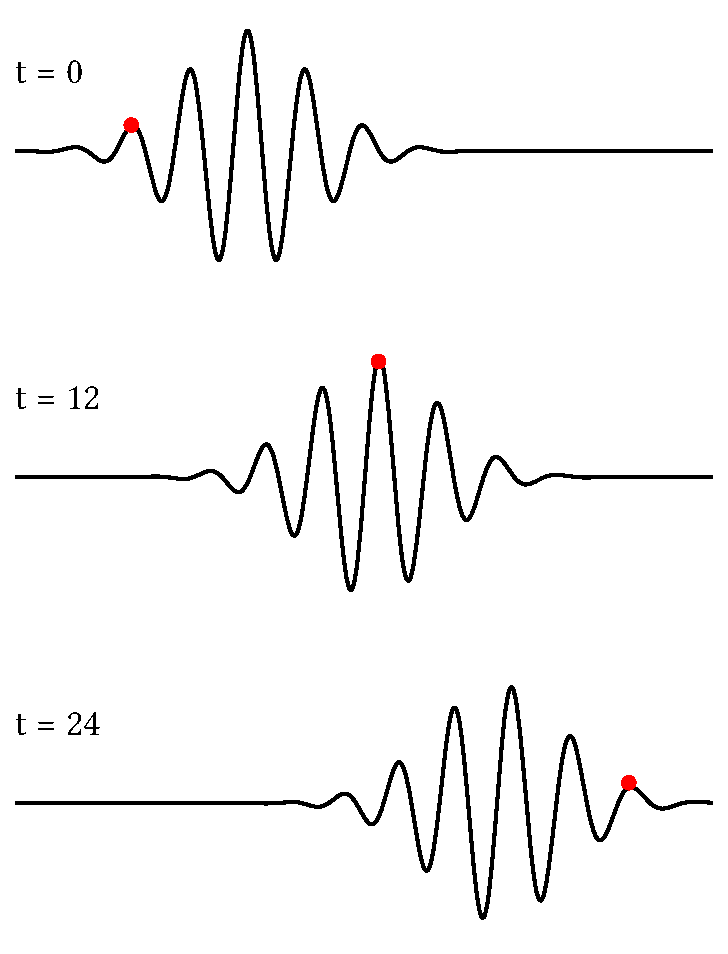
\includegraphics[width=0.6\linewidth]{Figures/Chapter5/fig_wave_packet_motion}
\caption{A wave packet in motion.  The dispersion relation is that for deep water waves, and the individual peaks in the wave packet (one is highlighted with the red dot) move twice as fast as the wave packet itself. The time units here are arbitrary.}
\label{fig_wave_packet_motion}
\end{figure}

% 5.2.3 - Energy and Group Velocity

\subsection{Group Velocity and Energy}

Perhaps not surprisingly when looking at wave motion like that shown in Figure \ref{fig_wave_packet_motion}, the energy in a wave is transported at the \emph{group velocity} $c_g$.  What is more surprising is that this is very general -- even our simple sinusoidal waves will transport energy at this speed rather than the phase speed, which is what the actual wave crests travel at.

We can show this easily enough, and while doing so explore the ideas of energy in fluids which we haven't touched on much.  For example, let's start with the kinetic energy.  The kinetic energy of a fluid element is of course
\[
T = \frac{1}{2} m \vec{u}^2,
\]
where $m = \rho \, d\tau$ is the mass of the element with infinitesimal volume $d\tau$ and $\vec{u}^2 = u^2 + v^2$ as usual.  The kinetic energy of some volume of the fluid requires an integral over the volume to add up the contributions from each element:
\begin{equation}
T = \frac{1}{2} \int \rho \vec{u}^2 \, d \tau.
\end{equation}
In our case, however, dealing with a two-dimensional fluid, we'll calculate the kinetic energy over an area $da = dx \, dy$, so that we'll have the kinetic energy per unit length in the $z$ direction.  We'll also only make use of one full wavelength as shown in Figure \ref{fig_wave_energy}. The kinetic energy is then
\begin{equation}
T = \frac{1}{2} \rho \int_{x_0}^{x_0 + \lambda} \int_{-\infty}^{\eta} (u^2 + v^2) \, dy \, dx.
\end{equation} 

Assuming a sinusoidal wave with a surface given by equation (\ref{eq_sin_eta}) and velocity potential by equation (\ref{eq_sin_pot}), you can show that the result is given by (see Problem \ref{prob_energy})
\begin{equation}
T = \frac{1}{4} \rho g A^2 \lambda.
\end{equation}
This is the kinetic energy (per unit length) in the fluid below one wavelength $\lambda$ of a sinusoidal surface wave.

\begin{figure}
\centering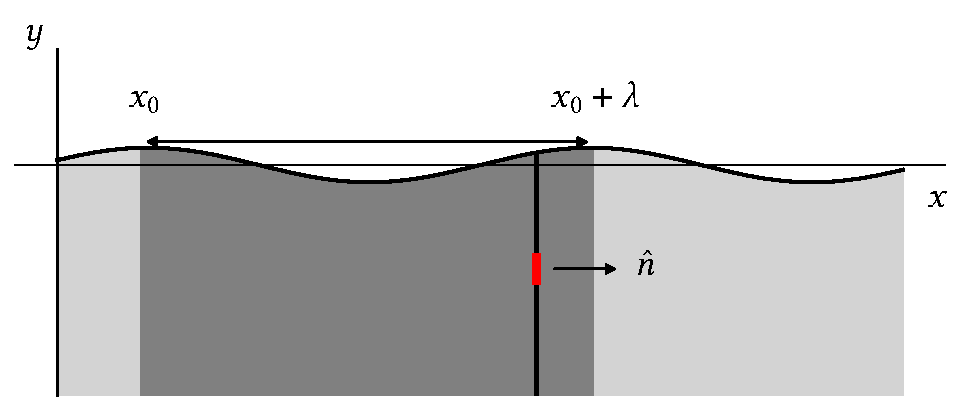
\includegraphics[width=0.8\linewidth]{Figures/Chapter5/fig_wave_energy}
\caption{We'll calculate the energy in the fluid within one wavelength.}
\label{fig_wave_energy}
\end{figure}

In addition, the fluid will have gravitational potential energy as it changes in height.  For a single fluid element, the potential energy is
\[
U = mgy,
\]
and integrating throughout the fluid gives
\begin{equation}
U = \int \rho g y d\tau.
\end{equation}
As with the kinetic energy, we'll only integrate over the area shown in Figure \ref{fig_wave_energy}, so the potential energy becomes
\begin{equation}
U = \int_{x_0}^{x_0 + \lambda} \int_{0}^{\eta} \rho g y \, dy \, dx.
\end{equation}
Notice that the lower bound for the inner integral is $y=0$ -- we're setting the zero-point of potential energy there.  For our sinusoidal waves, you can show (Problem \ref{prob_energy} again) the total potential energy in one wavelength of fluid is
\begin{equation}
U = \frac{1}{4} \rho g A^2 \lambda. 
\end{equation}
This is identical to the kinetic energy, and the total energy per unit length along $z$ is
\[
E = \frac{1}{2} \rho g A^2 \lambda.
\]
However, it's more customary to work with the total wave energy \emph{per wavelength,} or
\begin{equation}
\label{eq_wave_energy}
\bar{E} = \frac{1}{2} \rho g A^2.
\end{equation} 

We want to find the \emph{rate} at which this energy flows as the wave moves.  To do that, we'll calculate the \emph{power}, 
\[
P = \frac{dE}{dt} = \int d\vec{F} \cdot \vec{u}.
\]
Consider Figure \ref{fig_wave_energy} again.  The force of the fluid on a small area $da = dy dz$ (the red region) will be $d\vec{F} = p \ da \unit{x}$.  Now, as above, we'll make this calculation per unit length in the $z$ direction, so the power will be
\begin{equation}
P = \int_{-\infty}^\eta pu \, dy.
\end{equation}
The value of the pressure in this integral is that which is a result of the waves themselves, not the hydrostatic pressure due to gravity that was discussed in Section \ref{sec_static}.  We can find that from Euler's equation in the form of (\ref{eq_euler_wave}); rearranging for pressure (and dropping the quadratically small velocity term), it is
\begin{equation}
\frac{dE}{dt} = -\rho \dfdx{\varphi}{dt}.
\end{equation}
Substituting this and $u = \partial \varphi / \partial x$ into the integral, we get
\[
\frac{dE}{dt} = \frac{1}{2} \rho g \frac{\omega}{k} A^2 \cos^2(kx -\omega t).
\]
If we average this expression over one full period ($2\pi / \omega$) and use the phase speed, $c = \omega / k$, it becomes
\begin{equation}
\frac{d\bar{E}}{dt} = \frac{1}{4} \rho g A^2 c.
\end{equation}
This is the rate of energy transferred along the $x$ direction by the wave motion; notice that it's the \emph{average} energy.  But we calculated the average energy per wavelength above, and using equation (\ref{eq_wave_energy}) we can write
\[
\frac{d\bar{E}}{dt} = \bar{E} \left( \frac{1}{2} c \right)
\]
or, since the group speed is one half the phase speed,
\begin{equation}
\frac{d\bar{E}}{dt} = \bar{E} c_g.
\end{equation}

So, even in the case of pure sinusoidal waves, the energy is still transferred at the group speed rather than the phase speed.  It turns out this is actually a general result, valid for any dispersive  wave system.

% 5.2.4 - Long Time Response

\subsection{Long-Time Response}

Suppose there's some kind of disturbance in the middle of an otherwise calm pond.  Although the initial response of the water will be very complicated (top panel of Figure \ref{fig_long_response}), after enough time has passed and at a far enough distance from the disturbance, the wave structure will become more regular (bottom panels of Figure \ref{fig_long_response}).  This is because of \emph{dispersion} -- each Fourier sinusoidal component will travel at a particular speed, $c = \sqrt{g/k}$, according to its wavelength $\lambda = 2\pi/k$, with longer wavelengths travelling faster.  As you can see in Figure \ref{fig_long_response}, the wave has become approximately sinusoidal, but with a slowly varying wavelength, frequency, and amplitude.  At time $t_1$, far from the initial disturbance, the wavelength slowly increases.  A short time later at $t_2$, the wavelengths have become smaller in the same region.

\begin{figure}
\centering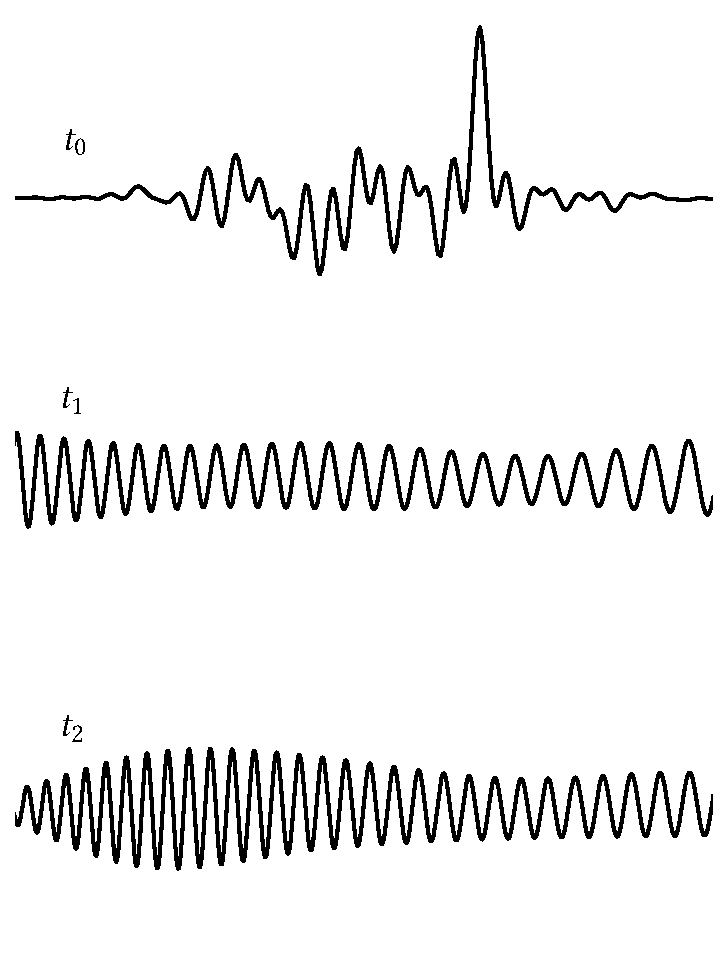
\includegraphics[width=0.7\linewidth]{Figures/Chapter5/fig_long_response}
\caption{An initially messy disturbance (top panel, $t_0$) will eventually become regular at long times and far distances (bottom panels, $t_1$ and $t_2$). }
\label{fig_long_response}
\end{figure}

Let's describe this long-time response to the disturbance by a \emph{local wavenumber} $k(x, t)$ and \emph{local frequency} $\omega(x, t)$.  We can then write for the surface the equation
\begin{equation}
\eta(x, t) = A(x, t) e^{i\theta(x, t)},
\end{equation}
where $A(x, t)$ describes the gradual modulation of the wave amplitude, and $\theta(x, t)$ the oscillatory aspect of it.  Presumably the amplitude is complicated and depends on the initial disturbance, but we can explore the oscillatory nature of the wave by connecting the function $\theta(x, t)$ to the local wavenumber and frequency.

To do that, consider first a single sinusoidal wave; in that case we'd have
\[
\theta(x, t) = kx - \omega t,
\]
as usual for a travelling wave.  That suggests we can write, in a more general sense,
\begin{equation}
k = \dfdx{\theta}{x}, \quad \text{and} \quad \omega = -\dfdx{\theta}{t}.
\end{equation}
Then note that 
\[
\dfdx{k}{t} = \frac{\partial^2 \theta}{\partial t \partial x} = -\dfdx{\omega}{x} = \frac{\partial^2 \theta}{\partial x \partial t},
\]
which means that
\begin{equation}
\label{eq_locals}
\dfdx{k}{t} + \dfdx{\omega}{x} = 0.
\end{equation}
But we know that the frequency is a function of wavenumber, $\omega = \omega(k)$, so
\[
\dfdx{\omega}{x} = \frac{d\omega}{dk}\dfdx{k}{x} = c_g \dfdx{k}{x},
\]
where I've used the group velocity $c_g = d\omega/dk$.  Equation (\ref{eq_locals}) then becomes
\begin{equation}
\label{eq_local_group}
\dfdx{k}{t} + c_g \dfdx{k}{x} = 0.
\end{equation}

This is a key result, although you may not recognize it.  Compare this equation to the definition of the material derivative,
\[
\frac{Df}{Dt} = \dfdx{f}{t} + (\vec{u} \cdot \grad ) f;
\]
they're the same, or would be if the velocity was purely in the $x$-direction.  Now, if $Df/Dt = 0$, then $f$ is constant for a particular fluid element.  If we apply that line of thought to the wave result, equation (\ref{eq_local_group}), it suggests that \emph{the local wavenumber $k(x, t)$ is constant for an observer moving with the group velocity $c_g$}.

\begin{example}[Deep water waves]
For deep water gravity waves, the dispersion relation is $\omega(k) = \sqrt{gk}$ and the group velocity is
\[
c_g = \frac{d\omega}{dk} \frac{1}{2} \sqrt{ \frac{g}{k} }.
\]
Our result above suggests that if we race along beside a wave with speed $c_g$, we'll always see the same wavenumber $k$ (or wavelength $\lambda$).

Let's pretend to do exactly that -- suppose a disturbance happens at $x=0$ and $t = 0$, and we start running (somehow on top of the water!) away from it with speed $c_g$.  After a time $t$ has passes, we're at position
\[
x = c_g t.
\]
Rearranging for the speed gives
\[
c_g = \frac{x}{t} = \frac{1}{2} \sqrt{ \frac{g}{k} },
\]
or
\begin{equation}
k = \frac{gt^2}{4x^2}.
\end{equation}
This equation tells us what wavenumber we'll see at position $x$ and time $t$.

Now, we also have
\begin{equation}
\omega = \sqrt{gk} = \frac{gt}{2x}.
\end{equation}
Returning to our idea of a local wavenumber and frequency, we can write
\[
\dfdx{\theta}{x} = k = \frac{gt^2}{4x^2} \quad \text{and} \quad \dfdx{\theta}{t} = -\omega = -\frac{gt}{2x}.
\]
Integrating gives
\begin{equation}
\theta(x, t) = -\frac{gt^2}{4x}
\end{equation}
(plus a constant which fixes the phase that I've dropped for simplicity), so the surface is given by
\begin{equation}
\label{eq_surface_reponse}
\eta(x, t) = A(x, t) e^{-i gt^2/4x}.
\end{equation}
The real part of this equation (for constant amplitude $A$) is plotted in Figure \ref{fig_local_wave_example} for two different times.  This surface matches what we saw in Figure \ref{fig_long_response}, which plotted the motion of a complicated wave packet; in both cases the wavenumber and frequency slowly change with time and space.
\end{example}

\begin{figure}
\centering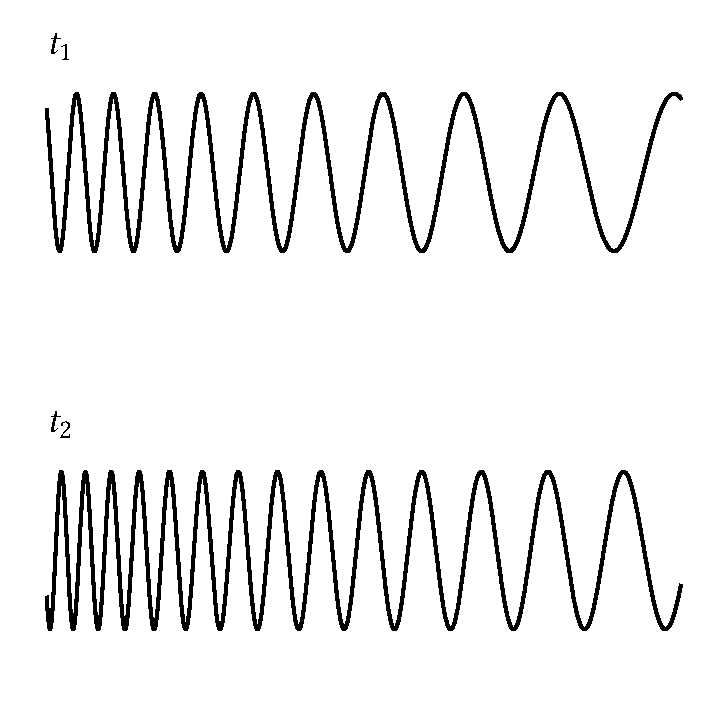
\includegraphics[width=0.7\linewidth]{Figures/Chapter5/fig_local_wave_example}
\caption{Equation (\ref{eq_surface_reponse}) plotted at two different long times, far from the disturbance at $x=0$.}
\label{fig_local_wave_example}
\end{figure}



%
%  SECTION 5.3 - Sound waves
%

\section{Sound Waves}

% 5.3.1 - Compressible Fluids

\subsection{Compressible Fluids}

% 5.3.2 - Small Amplitude Sound waves

\subsection{Small Amplitude Sound Waves}





\section*{Problems}
\addcontentsline{toc}{section}{Problems}
\markright{Problems}%

\begin{problem}[Effects of finite depth]
\label{prob_finite_depth}
To come
\end{problem}

\begin{problem}[Gravity-capillary dispersion relation]
\label{prob_grav_cap_dispersion}
To come
\end{problem}

\begin{problem}[Adding two cosines]
\label{prob_two_cosines}
To come
\end{problem}

\begin{problem}[Calculating energy]
\label{prob_energy}
To come
\end{problem}

